\documentclass[a4paper,ngerman]{atseminar}

\usepackage{microtype}
\usepackage{graphicx}
\usepackage{algorithm2e}
\usepackage[left]{lineno}
\usepackage{tikz}
\usetikzlibrary{bayesnet}
\usepackage{wasysym}
\usepackage{subfig}
\usepackage{tabularx}
\usepackage[final]{pdfpages}
\usepackage{float}

\setboolean{@twoside}{false}


\linenumbers

%% Please do not include packages that change the layout/size of the
%% of the document. They will be removed.

\bibliographystyle{plain}%the recommended bibstyle

% Preamble with header information 
\subject{Ausarbeitungen für das Seminar}
\title{Algorithmic Methods in the Humanities – Summer 2016}
% \titlerunning{Algorithmic Methods in the Humanities}%optional



\newcommand*{\vinput}[1]{\vcenter{\hbox{\input{#1}}}}
\newcommand*{\vpointer}{\vcenter{\hbox{\scalebox{2}{\Huge\pointer}}}}


%Organizer macros:%%%%%%%%%%%%%%%%%%%%%%%%%%%%%%%%%%%%%%%%%%%%%%%%%%%%%


%% do not use this field, but \summaryauthor
\author{}

%%%%%%%%%%%%%%%%%%%%%%%%%%%%%%%%%%%%%%%%%%%%%%%%%%%%%%%%%%%%%%%%%%%%%%%%%%%%%%%
%%%%%%%%%%%%%%%%%%%%%%%% begin of document %%%%%%%%%%%%%%%%%%%%%%%%%%%%%%%%%%%%
%%%%%%%%%%%%%%%%%%%%%%%%%%%%%%%%%%%%%%%%%%%%%%%%%%%%%%%%%%%%%%%%%%%%%%%%%%%%%%%
\begin{document}

\maketitle

%\GERMAN
\ENGLISH

%%%%% YOUR REPORT BEGINS HERE
\section{Latent Dirichlet Allocation}
\summaryauthor[Florian Becker]{Florian Becker}

\begin{abstract}
Due to the vast amounts of texts which are produced and digitized on a daily basis, it 
becomes more and more difficult to find what we are looking for. Topic models can 
be used as a tool to discover \textit{topics} in large collection of texts. Each text 
is considered to be a distribution over topics and topics are, in turn, distributions over
words. \\
Latent Dirichlet Allocation is a generative probabilistic topic model. The basic idea is
that documents are mixtures of latent topics distributed according to a Dirichlet prior.


\end{abstract}

\subsection{Introduction}
%"We are drowning in information but starved for knowledge." - John Naisbitt \\
When seeking digitized and hyper-linked information, we use searching tools that
weight each result according to some centrality measure. Such Techniques are 
often sufficient, provided that we only want to find some result and don't care
about the underlying topic structure which might give us more insight in a document or
even a collection of many documents.
Topic models enable us to not only search documents by the themes that they contain, but
also give us a tool with which we can automatically organize and structure text corpora.
It is assumed that a document exhibits multiple topics and each 
is a distribution over words. Consider, for instance, a corpus with texts about 
the digital humanities. A topic model algorithm might output that the text corpus
contains the topics \textit{Computer Science}, \textit{Linguistics} and \textit{Philosophy}.
But since every topic is a distribution over words, the algorithm won't just output '\textit{Computer Science}', 
but will rather give a distribution over words, which we then can identify as the topic '\textit{Computer Science}':
e.g. \textit{algorithm, program, complexity, machine, turing, artificial intelligence, etc}.
\\
Topic Models can also be thought of as a way of clustering similar documents.
Scientific papers, books, tweets, blogs can be organized according to the 
themes in them. With topic models organizing a large corpus becomes feasible. \\
Latent Dirichlet Allocation (LDA) is a generative topic model. That means, that 
the topic and word distribution of a document can be explained by a generative
model. In machine learning generative models are used \textit{simulate} data points.
The goal is to infer the hidden parameters which are assumed to be known in a 
generative model. Hence, inference can be seen as reversing the the generative 
process. In the case of Latent Dirichlet Allocation the hidden variables are the
per-document topic distribution, the per-document per-word topic assignments and
the topics themselves. \\
Latent Dirichlet Allocation was introduced by David Blei, Andrew Ng, and Michael Jordan in 2003 \cite{blei2003latent}.
Since then it has been applied in various different domains to many different sorts of texts:
For instance in the domain of public health,\cite{paul2011you} analyzed Tweets with LDA in order 
to track illnesses over time. LDA is not restricted to operate on 'classical' documents; it was also 
just recently applied in bioinformatics. \cite{pinoli2014latent} annotated genes with a feature term 
that describes a feature with LDA.
\\
As the intersection of computing and the humanities grows, topic models will become more important.
The humanities profit from algorithmic methodologies towards large text corpora for obvious reasons;
manually structuring those is not an option. Furthermore, the low-dimensional structure of a text corpus
might also give us insight about the semantic levels.
\\
After a section about preliminaries and notation this report will discuss the generative model, 
which can also be seen as a concise way to formulate the conditions of Latent Dirichlet Allocation.
Afterwards, the problem of Bayesian inference is discussed and a solution, the Gibbs Sampling algorithm, is presented.


\subsection{Preliminaries and Notation}

Throughout this report the notation of the original paper by Blei et al. will be used and 
is summarized in the following table.

\begin{table}[h]
\centering
\caption{Notation, as used in \cite{blei2003latent}.}
\begin{tabular}{l l}
\textbf{symbol} & \textbf{description} \\
 $\alpha$       & parameter of the Dirichlet prior on the per-document topic distributions \\
 $\beta$        & parameter of the Dirichlet prior on the per-topic word distribution \\ 
 $\theta_i$      & topic distribution for document i \\
 $\varphi_k$   & word distribution for topic k \\
 $z_{ij}$         & topic for the j th word in document i, and \\
 $w_{ij}$        & specific word.
  
\end{tabular}
\label{XY:tab:interesting}
% where X is the first letter of your first name and Y is the
% first letter of your last name.
\end{table}


In order to understand in what way topics are assumed to be distributed, the multinomial
and Dirichlet distribution including important properties will be shortly summarized.

\subsubsection{Multinomial Distribution}

The binomial distribution is a discrete distribution over events with two outcomes.
The probability mass function (PMF) is given by (\ref{binom}).

\begin{equation} \label{binom}
\Pr(X = k) = \binom n k  p^k(1-p)^{n-k}
\end{equation}

The binomial distribution is a special case of the multinomial distribution.
The multinomial distribution models events which have $k$ categories, 
where each has a fixed probability. The probability mass function is given by 

\begin{equation}
f(x_1,\ldots,x_k;n,p_1,\ldots,p_k) = { \displaystyle {n! \over x_1!\cdots x_k!}p_1^{x_1}\cdots p_k^{x_k}}
\end{equation}


\subsubsection{Dirichlet Distribution}
The Dirichlet distribution $Dir(\alpha)$ is a probability distribution parameterized by a positive real valued vector $\alpha$.
The probability density function is given by:

\begin{equation}
f \left(x_1,\cdots, x_{K}; \alpha_1,\cdots, \alpha_K \right) = \frac{\Gamma\left(\sum_{i=1}^K \alpha_i\right)}{\prod_{i=1}^K \Gamma(\alpha_i)} \prod_{i=1}^K x_i^{\alpha_i - 1}       \qquad\boldsymbol{\alpha}=(\alpha_1,\cdots,\alpha_K) 
\end{equation}

The Dirichlet distribution is often also expressed with the inverse of the Beta function as a normalizing constant.
${\mathrm{B}(\boldsymbol\alpha)}$ is constant as it only depends on the fixed parameter $\alpha$.

\begin{equation}
f \left(x_1,\cdots, x_{K}; \alpha_1,\cdots, \alpha_K \right) = \frac{1}{\mathrm{B}(\boldsymbol\alpha)} \prod_{i=1}^K x_i^{\alpha_i - 1}
\end{equation}

The expected value of the Dirichlet distribution is simply computed by:

\begin{equation}
\mathrm{E}[X_i] = \frac{\alpha_i}{\alpha_0}
\end{equation}
where 
\begin{equation}
\alpha_0 = \sum_{i=1}^K\alpha_i.
\end{equation}


The support of the Dirichlet distribution of order $K$ is the $(K-1)-$simplex. For $K=3$ the $2-$simplex is given by a
regular triangle, where each corner is an event. The vertices are  $(0,0,1), (0,1,0)$ and $(1,0,0)$.
A point $\vec{p} = (p_1,p_2,p_3)$ on this probability simplex corresponds to a certain event.
The Dirichlet distribution is \textit{conjugate} to the multinomial distributions, which means that 
for an observation coming from a multinomial distribution


\begin{figure}[!tbp]
  \centering
  \subfloat[$Dir(\alpha= \langle 2,1,1 \rangle)$]{\includegraphics[width=0.3\textwidth]{img/alpha211}\label{fig:f1}}
  \hfill
  \subfloat[$Dir(\alpha= \langle 2,2,2 \rangle)$]{\includegraphics[width=0.3\textwidth]{img/alpha222}\label{fig:f2}}
  \hfill
  \subfloat[$Dir(\alpha=\langle 10,10,10 \rangle )$]{\includegraphics[width=0.3\textwidth]{img/alpha101010}\label{fig:f3}}
  \hfill
  \caption{Dirichlet distributions in the two-dimensional simplex	 with different $\alpha$. The Corners $A$, $B$, $C$
  correspond to topics. More probable regions on the simplex are shown by a heat map, i.e. (dark) red corresponds to the
  most probable sample.}
\end{figure}



\subsection{Plate Notation}
In a probabilistic graphical model conditional dependence between various random variables are often depicted in plate notation.
Plate notation is a concise method for visualizing the factorization of the joint probability. 
Typically shaded nodes stand for \textit{observed} random variables.
The plates represent the repeated structure. 

\begin{figure}[H]
\centering
$\vinput{dependence_graph} \hspace{1cm }\vpointer  \hspace{1cm} \vinput{plate_dependence_graph}$
 \caption{Plate notation as a way to summarize conditional dependencies.}
  \label{fig:plate}
\end{figure}

The joint probability of the probabilistic graphical model depicted in (\ref{fig:plate}) is
\begin{align}
P[X_1,\ldots,X_n]=\prod_{i=1}^nP[X_i | parent(X_i)] = \prod_{i=1}^nP[X_i | Y]
\end{align}

The plate notation will be used in the next section to have a concise representation of
Latent Dirichlet Allocation and especially the conditional dependencies.

%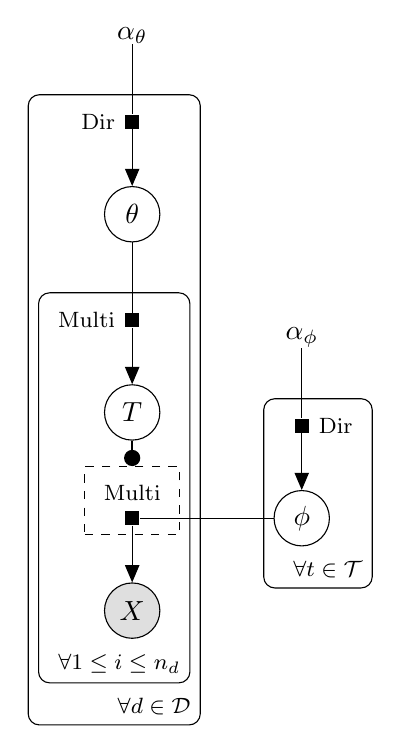
\begin{tikzpicture}[x=1.7cm,y=1.8cm]

  % Nodes

  \node[obs]                   (X)      {$X$} ; %
  \node[latent, above=of X]    (T)      {$T$} ; %
  \node[latent, above=of T]    (theta)  {$\theta$}; %
  \node[const, above=of theta] (atheta) {$\alpha_\theta$};


  % Factors
  \factor[above=of X]     {X-f}     {Multi} {} {} ; %
  \factor[above=of T]     {T-f}     {left:Multi} {} {} ; %
  \factor[above=of theta] {theta-f} {left:Dir} {} {} ; %

  % More nodes
  \node[latent, right=of X-f] (phi)  {$\phi$}; %
  \node[const, above=of phi]  (aphi) {$\alpha_\phi$}; %

  \factor[above=of phi] {phi-f} {right:Dir} {} {} ; %

  \factoredge {theta}  {T-f}     {T} ; %
  \factoredge {atheta} {theta-f} {theta} ; %
  \factoredge {phi}    {X-f}     {X} ; %
  \factoredge {aphi}   {phi-f}   {phi} ; %

  \gate {X-gate} {(X-f)(X-f-caption)} {T}

  \plate {plate1} { %
    (X)(X-gate) %
    (T)(T-f)(T-f-caption) %
  } {$\forall 1 \leq i \leq n_d$}; %
  \plate {} { %
    (plate1) %
    (theta)(theta-f)(theta-f-caption) %
  } {$\forall d \in \mathcal{D}$} ; %
  \plate {} { %
    (phi)(phi-f)(phi-f-caption) %
  } {$\forall t \in \mathcal{T}$} ; %

\end{tikzpicture}



\subsection{Generative Process}
Latent Dirichlet Allocation assumes the following generative process for
a corpus: \\

\begin{algorithm}[H]
\caption{Generative Model}
\KwIn{Dirichlet parameters $\alpha, \beta$}
\KwOut{$D$ documents (bag of words) with $N$ words}
1. Choose $ \theta_i \, \sim \, \mathrm{Dir}(\alpha) $,  \\
2. Choose $ \varphi_k \, \sim \, \mathrm{Dir}(\beta) $ \\
  \For{each word position $i,j$}{ %
   (a) Choose a topic $z_{i,j} \,\sim\, \mathrm{Multinomial}(\theta_i). $ \\
   (b) Choose a word $w_{i,j} \,\sim\, \mathrm{Multinomial}( \varphi_{z_{i,j}}) $
} %
\end{algorithm}
\vspace{1.5cm}

The generative model contains the main ideas of LDA. Data is treated as observations
coming from a process which samples words from a (hidden) distribution over topics.
Every word is generated independently from any other word. The generative process
does not take word order into account. Hence, the generative model is a produces a
bag of words, where order does not play a role. \\
If $3$ topics are chosen, e.g. \textit{Linguistics, Philosophy and Computer Science}, and if 
equal probability is given to all of them, then the generative process might produce 
bag-of-words resembling a text from \textit{Digital Humanities}. By putting more weight 
towards \textit{Linguistics} and \textit{Computer Science} the result would resemble 
documents from the domain of \textit{Computer Linguistics}.
The generative process of LDA is depicted as a bayesian probabilistic model in Figure \ref{fig:lda_plate}.

\begin{figure}[H]
\centering
\includegraphics[scale=0.55]{img/generative}
\caption{example}
  \label{fig:generative}
\end{figure}

In Figure \ref{fig:generative} the generative model is illustrated. The topic proportions are plotted
as a bar graph, the colored coins are the topic assignments for each word...



\begin{figure}[H]
\centering
\includegraphics[scale=0.35]{img/lda_plate}
 \caption{Plate notation for Latent Dirichlet Allocation corresponding to the generative process. Every vertex depicts a random variable.
 The shaded node $w_{d,n}$ stands for the observed words. Everything else is not observed and must be inferred.}
  \label{fig:lda_plate}
\end{figure}

\subsection{Experiments}
To fully grasp what LDA will produce as output, this section will provide an example with 
\textit{real world} data. \\
Gensim \footnote{ https://radimrehurek.com/gensim/index.html } is a tool for unsupervised semantic modelling.
The idea is to define three topics by using wikipedia articles. Then, all those wikipedia articles are
put in one corpus to see whether LDA can reproduce those the three original topics.

With gensim the model can be trained very easily: \\
lda = ldamodel.LdaModel(CORPUS, id2word$=$dictionary, num$\_$topics$=K$, update$\_$every$=1$, chunksize$=1$, passes $=350$)

\vspace{1.3cm}

\begin{tabular}{l l}
$\bullet$ computer science & \parbox[t]{10cm}{Algorithm, Computation, Computer Programming,  Programming Language\\ Computational complexity theory, Computability theory, Artificial Intelligence}\\  
\\
$\bullet$ philosophy & \parbox[t]{10cm}{Epistemology, Metaphysics, Continental philosophy, Ancient Greek,\\ Ethics, Aesthetics, Art, Phenomenology (philosophy), Pythagoras, Plato} \\
\\
$\bullet$ linguistics &  \parbox[t]{10cm}{Language, Semantics, Syntax, Phonology, Grammar,
               Phonetics, Pragmatics,  Corpus linguistics,\\
               Linguistic prescription, Linguistic description}
\end{tabular}

\vspace{1.3cm}

                               
The output of a call of LDA with $K=3$ is summarized in Table \ref{table:lda_output}.


\begin{table}[h!]
\caption{Each of the three topics is a distribution over the words. E.g. topic 1 resembles \textit{computer science}.}
\label{table:lda_output}
\begin{tabular}{l l l}
\textbf{TOPIC} & \textbf{PERCENTAGE} & \textbf{WORD} \\

1  &   0.010 & programming  \\
    &   0.009 & turing \\
    &   0.008 & problem \\
    &   0.007 & machine \\
    &   0.006 & problems \\
    &   0.006 & algorithms\\
    &   0.006 & algorithm  \\
    &   0.006 & set \\
    &   0.006 & complexity \\ 
    &   0.005 & time  \\
 \hline \\
 2 &  0.008 & plato \\
    &  0.006 & plato's  \\
    &  0.006 & knowledge \\ 
    &  0.005 & pythagoras \\
    &  0.005 & philosophy  \\
    &  0.004 & phenomenology \\
    &  0.004 & greek  \\
    &  0.004 & according  \\ 
    &  0.004 & socrates  \\
    &  0.003 & theory \\
  \hline \\
3 & 0.019 & language \\
   & 0.009 & languages  \\
   & 0.007 & art \\
   & 0.005 & meaning \\ 
   & 0.005 & linguistic \\
   & 0.005 & human \\
   & 0.004 & ethics \\
   & 0.004 & speech \\
   & 0.004 & study \\
   & 0.004 & grammar 
\end{tabular}
\end{table}


Given a set corpus of wikipedia articles, LDA finds three topics which resemble the topics \textit{computer science},
\textit{philosophy} and \textit{linguistics}. 


\begin{figure}
\centering
\includegraphics[scale=0.4]{img/experiment}
 \caption{}
   \label{fig:experiments}
\end{figure}

\subsection{(Bayesian) Inference}

Inference means computing the \textit{posterior} and corresponds to '\textit{reversing}' the generative model.
In other words, inference is about fitting a generative model (the hidden parameters), such that it explains the observed data.

Many methods solving the problem of maximum aposterior estimation have been proposed. The original paper on LDA \cite{blei2003latent} suggested a Variational Bayesian method which can be understood as an extension of the expectation-maximization algorithm \cite{fox2012tutorial}. Gibbs Sampling as a way to compute the
posterior was proposed by Steyvers and Griffiths \cite{steyvers2007probabilistic}	 \\




\begin{align*} \label{post}
p(\beta_{1:K}, \theta_{1:D}, z_{1:D} | w_{1:D} ) = \frac{p(\beta_{1:K}, \theta_{1:D}, z_{1:D},w_{1:D} )}{p(w_{1:D})}
\end{align*}

The posterior is intractable to compute. More precisely, the denominator of (\ref{post}), the marginal probability, is not feasible to 
compute. To compute $p(w_{1:D})$ one would have to sum the joint distribution over all possible instances of the hidden topic structure.



\subsubsection{Gibbs Sampling}

Gibbs Sampling, named after the physicist Josiah Willard Gibbs, is a Markov Chain Monte Carlo Algorithm (MCMC) and can be used to approximate the marginal and posterior 
distribution by constructing a Markov chain which converges to the target distribution.
A Markov chain represent a random process, where going from one state to another is determined by a transition matrix.
An entry $p_{i,j}$ corresponds to the probability of going from state $i$ to state $j$.

With Gibbs Sampling the goal is to integrate out the per document topic proportions $\theta$.

In order to assign a word to a topic, the Gibbs sampler computes the probability of a topic $z_d,n$ if it is assigned to a word $w_d,n$, where 
all other word-to-topic assignments are given or fixed. $z_{\textunderscore_ {d,n}}$ is defined to be the notation for all topic assignments except 
for for $z_{d,n}$ \\
Formally:

\begin{equation} \label{eq:gibbs}
p(z_{d,n} = k | z_{\textunderscore_ {d,n}},w,\alpha, \beta) = \frac{p(z_{d,n}=k, z_{\textunderscore_ {d,n}} | w, \alpha, \beta)}{p(z_{\textunderscore_ {d,n}} | w,\alpha, \beta)}
\ref{}
\end{equation}

It was shown \cite{griffiths2004finding} that equation \ref{eq:gibbs} can be calculated by:

\begin{equation} \label{eq:gibbs_}
p(z_{d,n} = k | z_{\textunderscore_ {d,n}},w,\alpha, \beta) \propto \frac{C_{n,k}^{WT}+\beta}
{\sum_{n=1}^{W}C_{n,k}^{WT}+W\beta} \cdot \frac{C_{d,k}^{DT}+\alpha}{\sum_{t=1}^{T}C_{d,t}^{DT}+T\alpha}
\end{equation}

$C_{n,k}^{WT}$ and $C_{d,k}^{DT}$ are matrices. $C_{n,k}^{WT}$ is the number of times topic $k$ was assigned to 
word $n$. On the other hand $C_{d,k}^{DT}$ is the number of times topic $k$ was assigned to words in document $d$.

The first step of the Gibbs Sampling algorithm is to randomly assign every word of all documents to a topic. By this 
the count matrices $C_{n,k}^{WT}$ and $C_{d,k}^{DT}$ are filled with values.
Gibbs Sampling will now sample topic assignments according to \ref{eq:gibbs_}.

The first term of the product in \ref{eq:gibbs_} also corresponds to an estimate of $\varphi_i$, 
and the second therm to an estimate of $\theta_j$

\begin{equation}
\hat{\varphi_i} = \frac{C_{i,j}^{WT}+\beta} {\sum_{k=1}^{W}C_{k,j}^{WT}+W\beta}
\end{equation}

\begin{equation}
\hat{\theta_j} = \frac{C_{d,j}^{DT}+\alpha}{\sum_{t=1}^{T}C_{d,t}^{DT}+T\alpha}
\end{equation}




\begin{example}
The following step-by-step example illustrates how Gibbs Sampling can be used to assign a topic to a word.
Consider the sentence (which represents one document out of a corpus):

\vspace{1cm}
\textit{Text mining algorithms can be used to find structure in text corpora like Plato’s $dialogues$}
\vspace{1cm}

Apriori we choose the number of topics $K=3$
\\
The first step is to remove stop words and randomly assign each word to a topic randomly. This is done to all documents.
\\
\begin{table}[h]
\centering
\caption{Tables have headers.}
\begin{tabular}{| c | c | c | c | c | c | c | }
\hline
1 & 3 & 2 & 1 & 2 & 1 & 2 \\
\hline 
text & mining & algorithms & structure & corpora & Plato & dialogues \\
\hline
\end{tabular}
\end{table}

The counts for all documents:
\\ \\
\begin{table}[h]
\centering
\caption{(random) word counts for every topic}
\begin{tabular}{ l | c l c | c  }
& \textbf{1} & \textbf{2} & \textbf{3} \\
\hline 
text & 65 & 54 & 59 \\
mining &  21 & 4 & 12 \\
algorithms & 100 & 74 & 122 \\
structure & 20 & 12 & 14 \\
corpora &  5 & 2 & 12 \\
Plato &  35 & 33 & 42 \\
dialogues &  24 & 27 & 31 \\
\end{tabular}
\end{table}

The goal is now to resample the word \textit{algorithm}.

\begin{table}[h]
\centering
\caption{Tables have headers.}
\begin{tabular}{ | c | c | c | c | c | c | c |}
\hline
1 & 3 & ??? & 1 & 2 & 1 & 2 \\
\hline
text & mining & algorithms & structure & corpora & Plato & dialogues \\
\hline
\end{tabular}
\end{table}

The assignment of the word \textit{algorithm} is determined by sampling according
to the topic distribution in the document and the word distribution over the corpus.
In Figure \ref{fig:topics_distr} the sampling is depicted. The blue bars correspond to 
the topic distribution, the yellow bars to the word distribution over topics.
Accordingly, it is most likely that \textit{algorithm} is assigned to topic 1, since the green 
area for topic 1 is the largest.

\begin{figure}[H]
\centering
\includegraphics[scale=0.30]{img/topics_distr}
 \caption{}
  \label{fig:topics_distr}
\end{figure}

According to the above 

\end{example}





\subsection{Conclusion}

Topic models enable scholars to find the hidden topic structure in large text 
corpora. The hidden structure must be uncovered in order to gain information 
about the low-dimensional structure behind a text corpus.
A topic modeling algorithm takes a corpus as an input and will output the topics
running through that corpus.

Reversing the generative model by applying gibbs sampling yields a solution of 
the inference problem.












\bibliography{references}



%%%%% YOUR REPORT ENDS HERE




\end{document}
